\documentclass{article}

% these packages let you do math
\usepackage{amsmath}
\usepackage{amssymb}

% we need these packages for fancy R tables
\usepackage{booktabs}
\usepackage{float}
\usepackage{colortbl}
\usepackage{xcolor}

% these packages play with the spacing/margins of the document. Uncomment the commands on lines 16 and 17 to see what they do.
\usepackage{a4wide}
\usepackage{setspace}
\usepackage{geometry}
\usepackage{parskip}
%\doublespacing
%\geometry{margin=1.5in}

% this package helps us with including images. Setting the graphics path makes it easier to refer to things in the \includegraphics command.
\usepackage{graphicx}
\graphicspath{ {../figures/} }

% make some hyperlinks using the \href command
\usepackage{hyperref}
\hypersetup{
    colorlinks=true,
    linkcolor=black,
    urlcolor=blue
}

% set the author, title, and date of the document. \maketitle adds it to the document.
\author{Jacob Bulzak}
\title{My Paper on NLSY97 Data}
\date{February 2022}

\begin{document}
\maketitle

\section{Introduction}

In this report we examine patterns in incarceration status by race and gender using the NLSY97 data from the year 2002. The analysis involved examining the incarceration status of individuals in the dataset and tracking the mean number of months incarcerated for the year 2002 based on race and gender. We note that the average number of months incarcerated tends to be very low, as the majority of survey respondents were not incarcerated at all for the year 2002.

We run the following regression:

\begin{equation*}
    y = \beta_1 + \beta_2 Hispanic + \beta_3 Mixed Race (Non-Hispanic)+ \beta_4 Non-Black / Non-Hispanic + \beta_5 Male + \varepsilon
\end{equation*}

\section{Analysis}


\begin{figure}[H]
    \begin{center}
        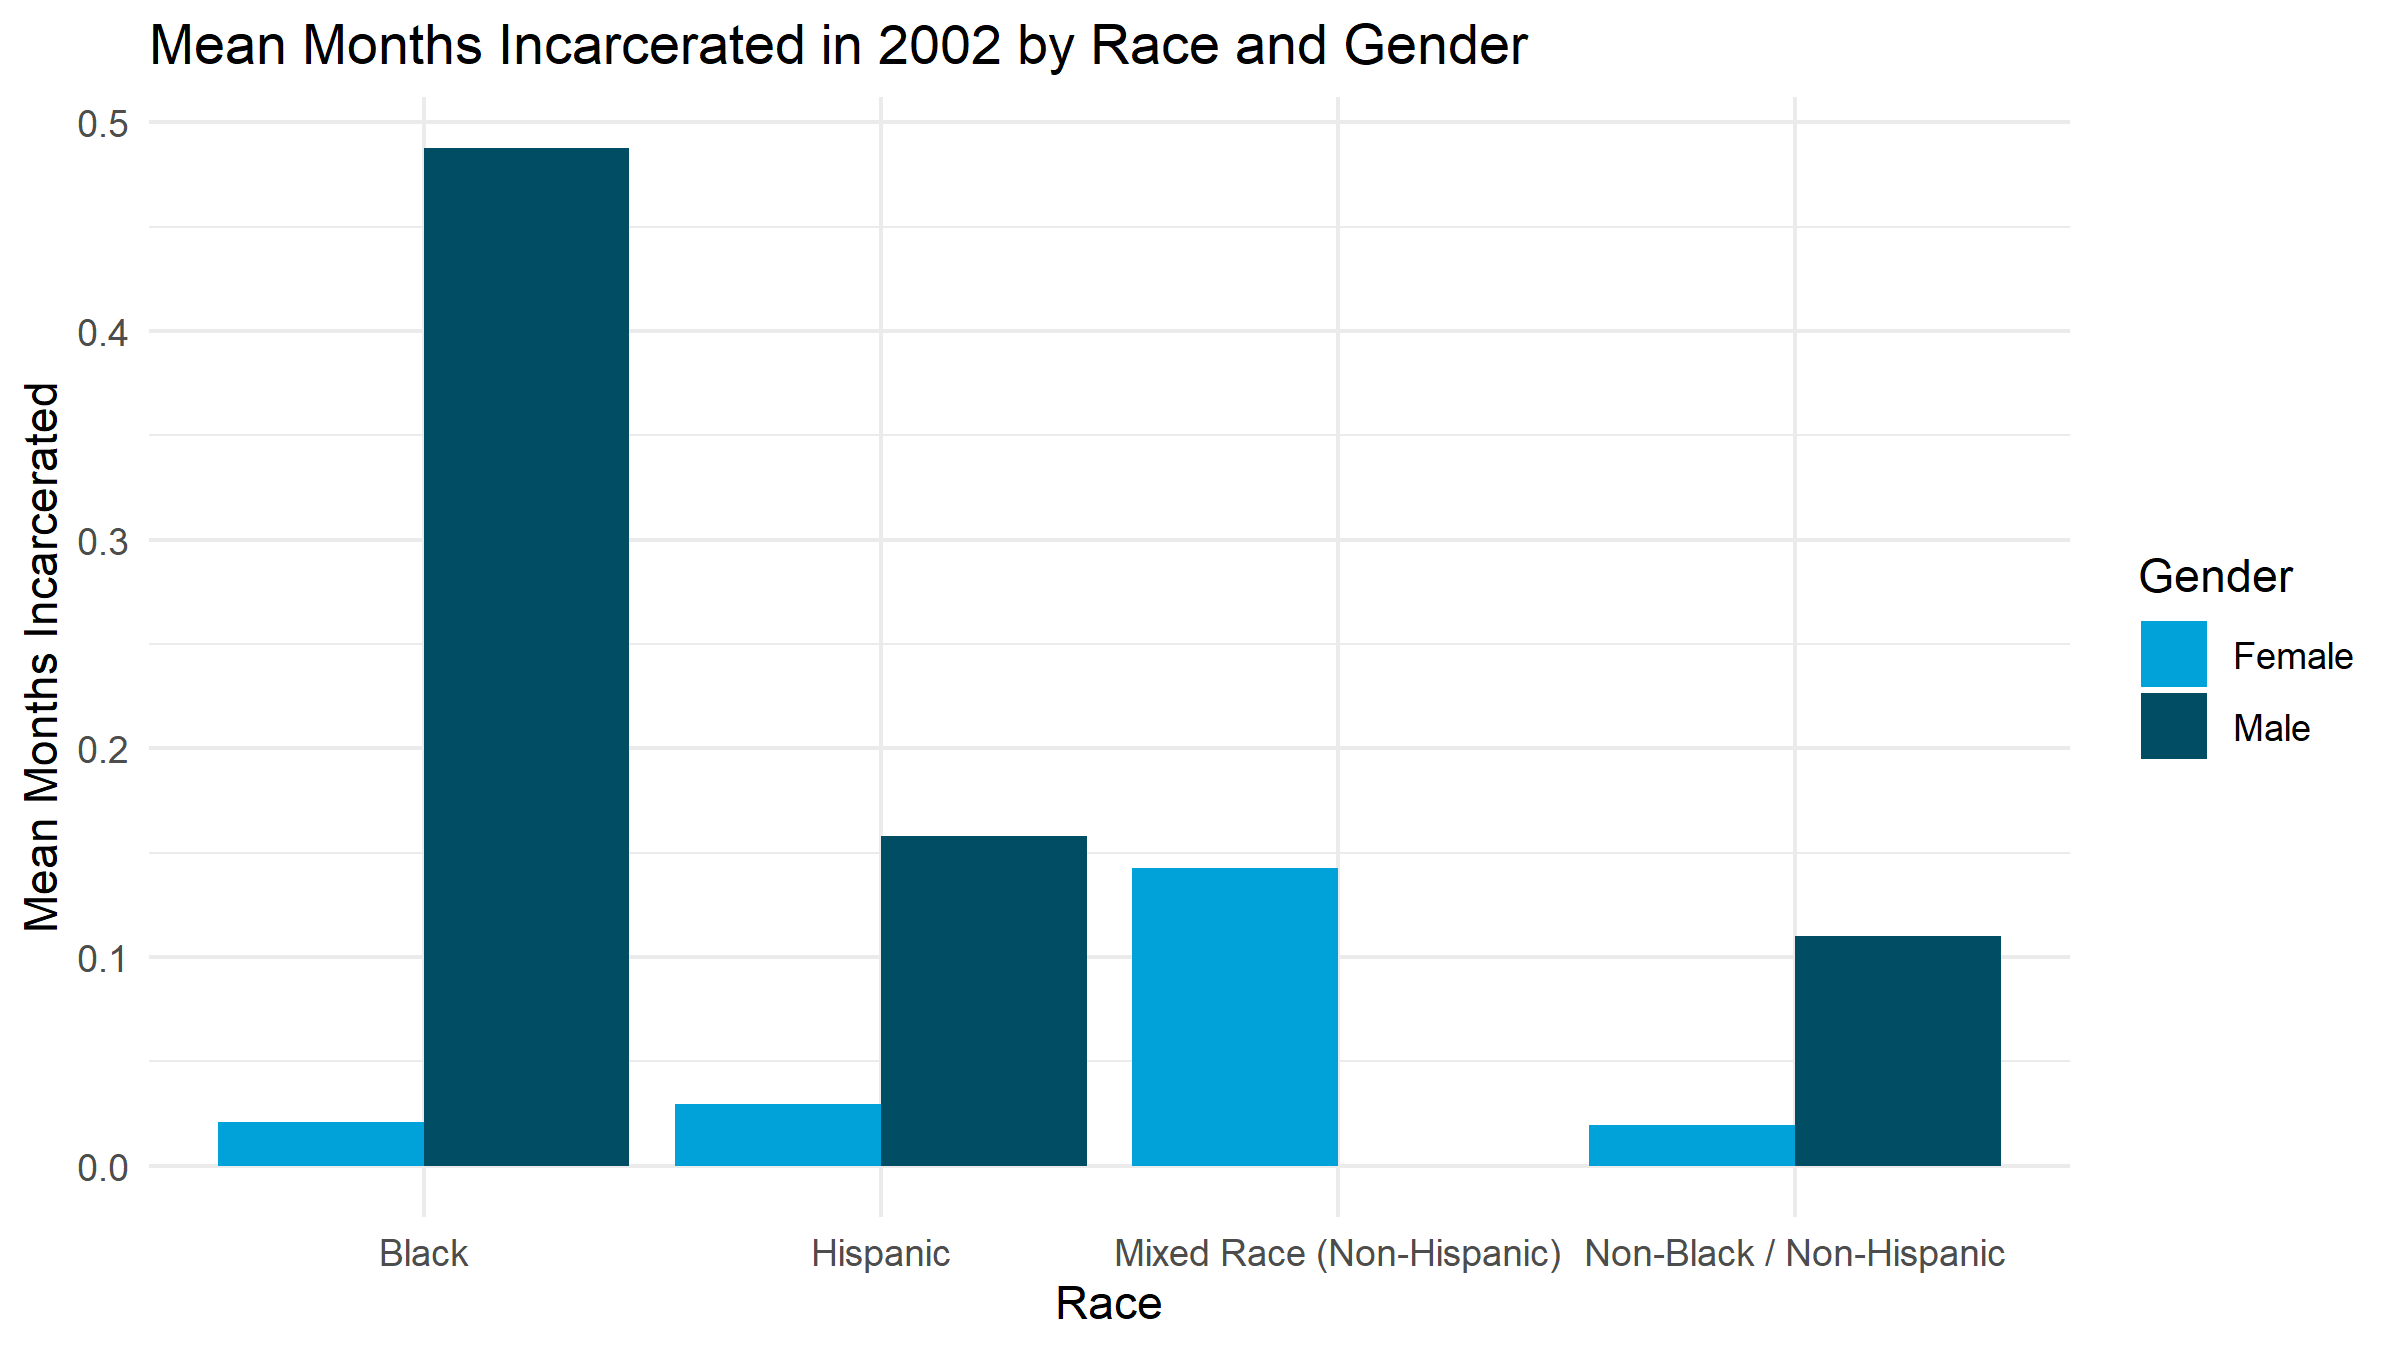
\includegraphics[width=.85\textwidth]{incarcerated_by_racegender}
    \end{center}
    \caption{Mean Number of Months Incarcerated in 2002 by Race and Gender}
    \label{fig:graph}
\end{figure}

The above graph shows the mean number of incarcerations in 2002 by race and broken down by gender. In every category, (except for Mixed Race (Non-Hispanic)) the mean number of months incarcerated is higher for males than for females. In fact, Mixed Race Non-Hispanic males have a mean incarceration time of zero months. Finally, we observe that the average duration of incarceration for Black males is much higher than for any other category.

\begin{table}[H]

\caption{\label{tab:tab:summarystats}Mean Months Incarcerated in 2002 by Race and Gender}
\centering
\begin{tabular}[t]{lrrrr}
\toprule
Gender & Black & Hispanic & Mixed Race Non Hispanic & Non Black Non Hispanic\\
\midrule
\cellcolor{gray!6}{Female} & \cellcolor{gray!6}{0.0211268} & \cellcolor{gray!6}{0.0298013} & \cellcolor{gray!6}{0.1428571} & \cellcolor{gray!6}{0.0193192}\\
Male & 0.4876712 & 0.1579509 & 0.0000000 & 0.1099476\\
\bottomrule
\end{tabular}
\end{table}


Table 1 serves as numeric representation of Figure 1. The table reiterates the results seen in the graph above: Black males exhibit the maximum mean incarceration time, whereas Mixed Race Non-Hispanic males zero months incarcerated in 2002, on average.


% Table created by stargazer v.5.2.2 by Marek Hlavac, Harvard University. E-mail: hlavac at fas.harvard.edu
% Date and time: Fri, Feb 18, 2022 - 10:08:25 PM
\begin{table}[!htbp] \centering 
  \caption{Regression Output. Omitted category is Black Females.} 
  \label{tab:regression} 
\begin{tabular}{@{\extracolsep{5pt}}lc} 
\\[-1.8ex]\hline 
\hline \\[-1.8ex] 
 & \multicolumn{1}{c}{\textit{Dependent variable:}} \\ 
\cline{2-2} 
\\[-1.8ex] & Months Incarcerated in 2002 \\ 
\hline \\[-1.8ex] 
 Hispanic & $-$0.159$^{***}$ \\ 
  & (0.038) \\ 
  & \\ 
 Mixed Race (Non-Hispanic) & $-$0.174$^{**}$ \\ 
  & (0.083) \\ 
  & \\ 
 Non-Black / Non-Hispanic & $-$0.189$^{***}$ \\ 
  & (0.035) \\ 
  & \\ 
 Male & 0.194$^{***}$ \\ 
  & (0.022) \\ 
  & \\ 
 Constant & 0.155$^{***}$ \\ 
  & (0.026) \\ 
  & \\ 
\hline \\[-1.8ex] 
Observations & 8,621 \\ 
R$^{2}$ & 0.015 \\ 
Adjusted R$^{2}$ & 0.014 \\ 
Residual Std. Error & 1.019 (df = 8616) \\ 
F Statistic & 32.033$^{***}$ (df = 4; 8616) \\ 
\hline 
\hline \\[-1.8ex] 
\textit{Note:}  & \multicolumn{1}{r}{$^{*}$p$<$0.1; $^{**}$p$<$0.05; $^{***}$p$<$0.01} \\ 
\end{tabular} 
\end{table} 


Table 2 summarizes the results of a the regression introduced in Section 1 that relates race and gender to incarceration time. We note that the model's coefficient of determination (i.e. R-squared) is 0.015. This indicates only a very small proportion of the variation in incarceration time is predictable from our covariates, implying a poor model fit. Conversely, each of the p-values associated with the covariate coefficients is significant at the 1 percent level. This tell us that changes in race and gender are indeed associated with changes in incarceration time, and furthermore, that these covariates belong in our regression. The table also demonstrates being Black is the greatest contributor to incarceration time given that it is the omitted variable in our regression and all other races have negative coefficients associated with them. Specifically, being a black male corresponds to, on average, a 0.194-month increase in time incarcerated. Finally, we note that the regression intercept (constant) represents the average number of months incarcerated for a Black female.


\end{document}

